\documentclass{beamer}
\usetheme{Madrid}

\title{Perceptron}
\author{Your Name}
\date{\today}

\begin{document}

\begin{frame}
    \titlepage
\end{frame}

\begin{frame}
    \frametitle{Characteristics of Biological Neural Networks}
    \begin{itemize}
        \item[(a)] \textbf{Highly interconnected:} Neurons form a complex web of connections.
        \item[(b)] \textbf{Robustness and Fault Tolerance:} The decay of nerve cells does not affect the overall function of the network significantly.
        \item[(c)] \textbf{Flexibility:} The ability to reorganize and adapt to new situations.
        \item[(d)] \textbf{Handling incomplete information:} Ability to infer appropriate outputs even when some inputs are missing or noisy.
        \item[(e)] \textbf{Parallel processing:} Multiple neurons can process information simultaneously.

    \end{itemize}
\end{frame}

\begin{frame}{Neuron structure}
    \begin{figure}
        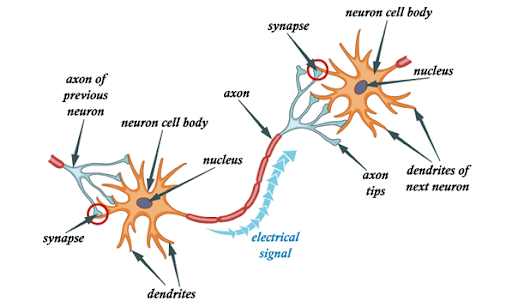
\includegraphics[width=0.8\linewidth]{figures/biological_neuron.png}
        \caption{Structure of a biological neuron}
    \end{figure}
\end{frame}

\begin{frame}{Neuron structure}
    \begin{itemize}
        \item Fundamental unit: neuron (cell body / soma, dendrites, axon, synapses).
        \item Dendrites receive inputs; axon transmits output and branches to many synapses (often thousands).
        \item Synapse: junction between axon terminal and target cell.
        \item Synaptic junctions form between presynaptic axon terminals and postsynaptic dendrites or the cell body.
        \item Typical sizes: soma ~ $10$--$80\ \mu$m; synaptic gap ~ $200\ \mathrm{nm}$; neuron length from $0.01\ \mathrm{mm}$ to $1\ \mathrm{m}$.
    \end{itemize}
\end{frame}

\begin{frame}{Signal transmission and firing}
    \begin{itemize}
        \item Resting potential ~ $-70\ \mathrm{mV}$; depolarization above threshold (roughly $\!\sim10\ \mathrm{mV}$) triggers firing.
        \item Action potentials are all-or-none pulses sent down the axon; information is encoded in firing rate (~1--100 Hz).
        \item Propagation speed in brain tissue ~ $0.5$--$2\ \mathrm{m/s}$; synaptic transmission delay ~ $0.5\ \mathrm{ms}$.
        \item After firing the membrane recovers (refractory period); synaptic effects decay with time constant ~$5--10\ \mathrm{ms}$.
    \end{itemize}
\end{frame}

\begin{frame}{Synapses: chemistry and types}
    \begin{itemize}
        \item Transmission across synapse is chemical: neurotransmitters released from presynaptic terminal.
        \item Postsynaptic effect can be excitatory (depolarizing) or inhibitory (hyperpolarizing).
        \item All endings of a given axon are typically either excitatory or inhibitory.
        \item Synaptic strength depends on activity and can change over time (basis for learning).
    \end{itemize}
\end{frame}

\begin{frame}{Plasticity and learning}
    \begin{itemize}
        \item Active synapses that repeatedly contribute to postsynaptic firing tend to strengthen; inactive ones weaken.
        \item Hebb's rule (``cells that fire together, wire together'') describes this activity-dependent plasticity.
        \item Continuous modification of synaptic strengths underlies learning and memory formation.
    \end{itemize}
\end{frame}

\begin{frame}{Network-scale properties}
    \begin{itemize}
        \item Convergence/divergence: neurons receive many inputs and send outputs to many others.
        \item Average inputs per neuron: on the order of $10^{4}$ synapses; total synaptic connections in human brain estimated ~$\sim10^{15}$.
        \item The cortex contains extremely dense, layered networks with vast numbers of interconnected neurons.
        \item Studying simple, identical units helps understand complex brain functions, but full understanding remains far off.
    \end{itemize}
\end{frame}

\begin{frame}{Key takeaways}
    \begin{itemize}
        \item Neurons are simple units whose structure (dendrite/axon/synapse) enables complex computation.
        \item Signals are electrical within neurons and chemical at synapses; timing and rate carry information.
        \item Synaptic plasticity provides a biological basis for learning (Hebbian adaptation).
        \item Massive connectivity (many synapses per neuron, ~$10^{15}$ total) creates powerful, distributed processing.
    \end{itemize}
\end{frame}

\end{document}